% scratch tex file for trying out stuff for presentation.

% This text is proprietary.
% It's a part of presentation made by myself.
% It may not used commercial.
% The noncommercial use such as private and study is free
% May 2007
% Author: Sascha Frank 
% University Freiburg 
% www.informatik.uni-freiburg.de/~frank/
%
% 
\documentclass{beamer}
\setbeamertemplate{navigation symbols}{}

\usepackage{beamerthemeshadow}


% added JW:
\usepackage{amsmath}




\begin{document}
\title{SiScLab Project 8}  
\author{Katta, Partmann, Wasmer}
\date{\today} 

% \begin{frame}
% \titlepage
% \end{frame}

\section{Implementation}
\label{sec:implementation}

\begin{frame}\frametitle{Module Design}
    TODO \texttt{hdf} preprocessor as self-contained module built for extension
    
    TODO \texttt{plot} visualization common to all frontends
    
    TODO \texttt{tk, jupyter} 2 interactive frontends (deployment)
\end{frame}

\subsection{Preprocessor}
\label{sec:preprocessor}

\begin{frame}
    \frametitle{Preprocessor Module}
    HDF is a hierarchical format for scientific data.

    TODO Image \texttt{hdf} Flow Diagram

    \begin{itemize}
    \item modular output types
    \item dependency resolution
    \end{itemize}
\end{frame}

\begin{frame}
    \frametitle{Preprocessing}

    TODO explain main part \texttt{get\_data}.
    
    \begin{displaymath}
        \tilde{W}^{\text{eff}}_{skn} = \frac{\sum\limits_{\substack{g \in \text{groups} \\ c \in \text{characters}}} L_{skngc} G_g}{\sum\limits_{\substack{g \in \text{all groups} \\ c \in \text{all characters}}} L_{skngc} G_g}
    \end{displaymath}

    TODO explain optimizations (this may need 2 slides):
    \begin{itemize}
    \item reshaping
    \item weight filter
    \item tensor?
    \item buffering
    \end{itemize}
\end{frame}

\subsection{Interactive Visualization}
\label{sec:visualization}

\newcommand{\theimage}{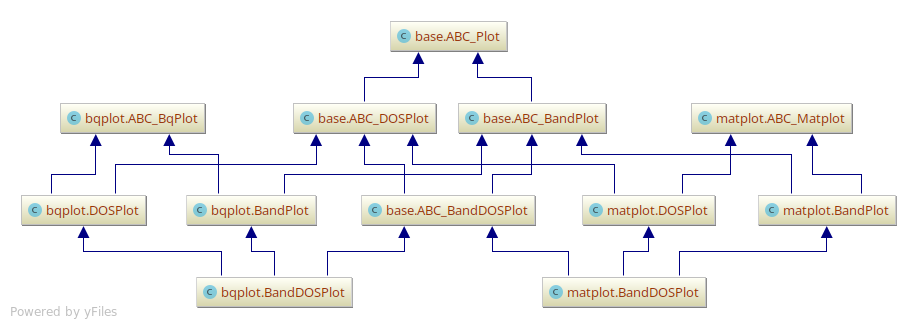
\includegraphics[width=1.1\linewidth]{img/pycharm_uml/matplot.png}}% Shorthand
\begin{frame}\frametitle{Visualization Module}
    \begin{itemize}
    \item Abstract interfaces for different viz. libs and applications
    \item \texttt{InteractiveControlDisplay} as frontend contracts 
    \end{itemize}    
    \centerline{\theimage}
\end{frame}

\subsection{Desktop Frontend}
\label{sec:desktop-frontend}

\begin{frame}\frametitle{Desktop Frontend}
    TODO Praneeth?
\end{frame}

\subsection{Web Frontend}
\label{sec:web-frontend}

\begin{frame}\frametitle{Web Frontend}
    TODO Selection Process from Notes 
\end{frame}

\begin{frame}\frametitle{}
    TODO Selection Process Choices from Notes 
\end{frame}







\end{document}



%%% Local Variables:
%%% mode: latex
%%% TeX-master: t
%%% End:
